\thispagestyle{toancuabinone}
\pagestyle{toancuabi}
\everymath{\color{toancuabi}}
%\blfootnote{$^1$\color{toancuabi}Đại học Thăng Long.}
\graphicspath{{../toancuabi/pic3/}}
\begingroup
\AddToShipoutPicture*{\put(0,616){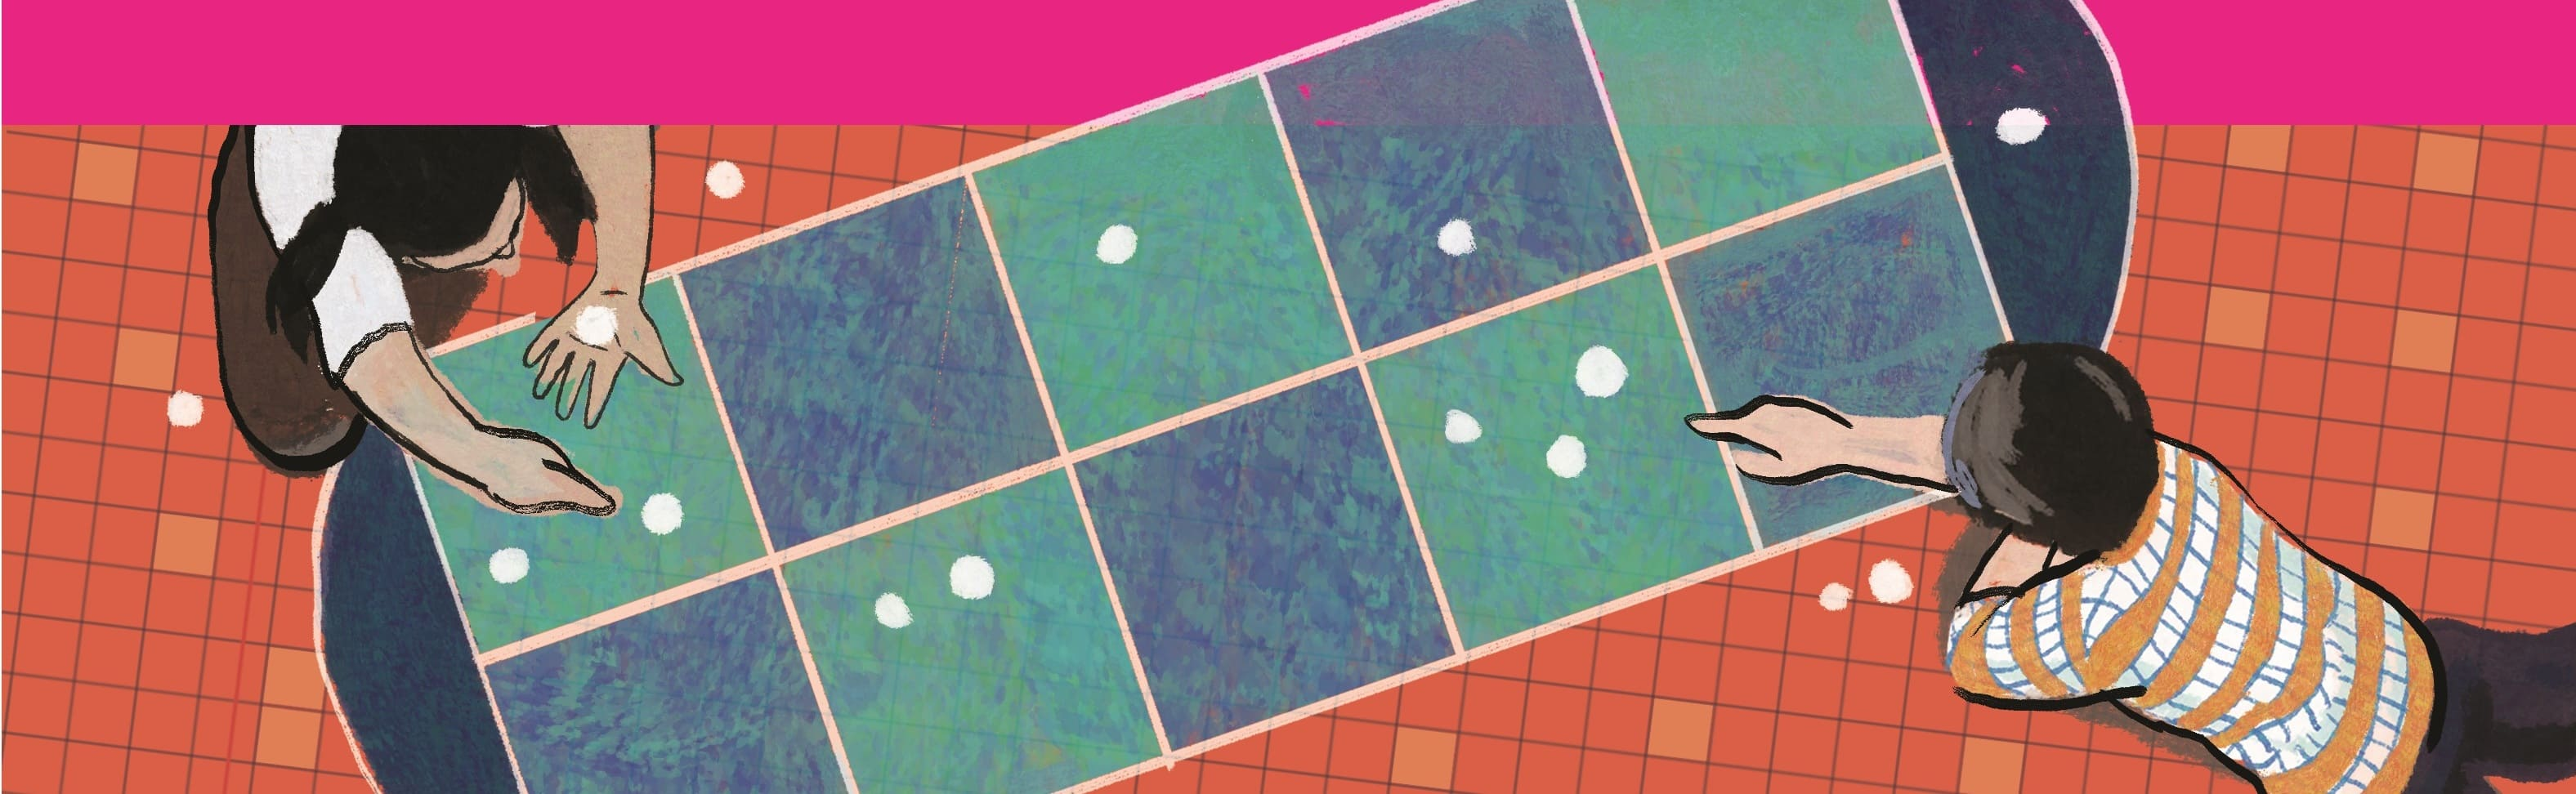
\includegraphics[width=19.3cm]{../bannertoancuabi}}}  
\AddToShipoutPicture*{\put(90,550){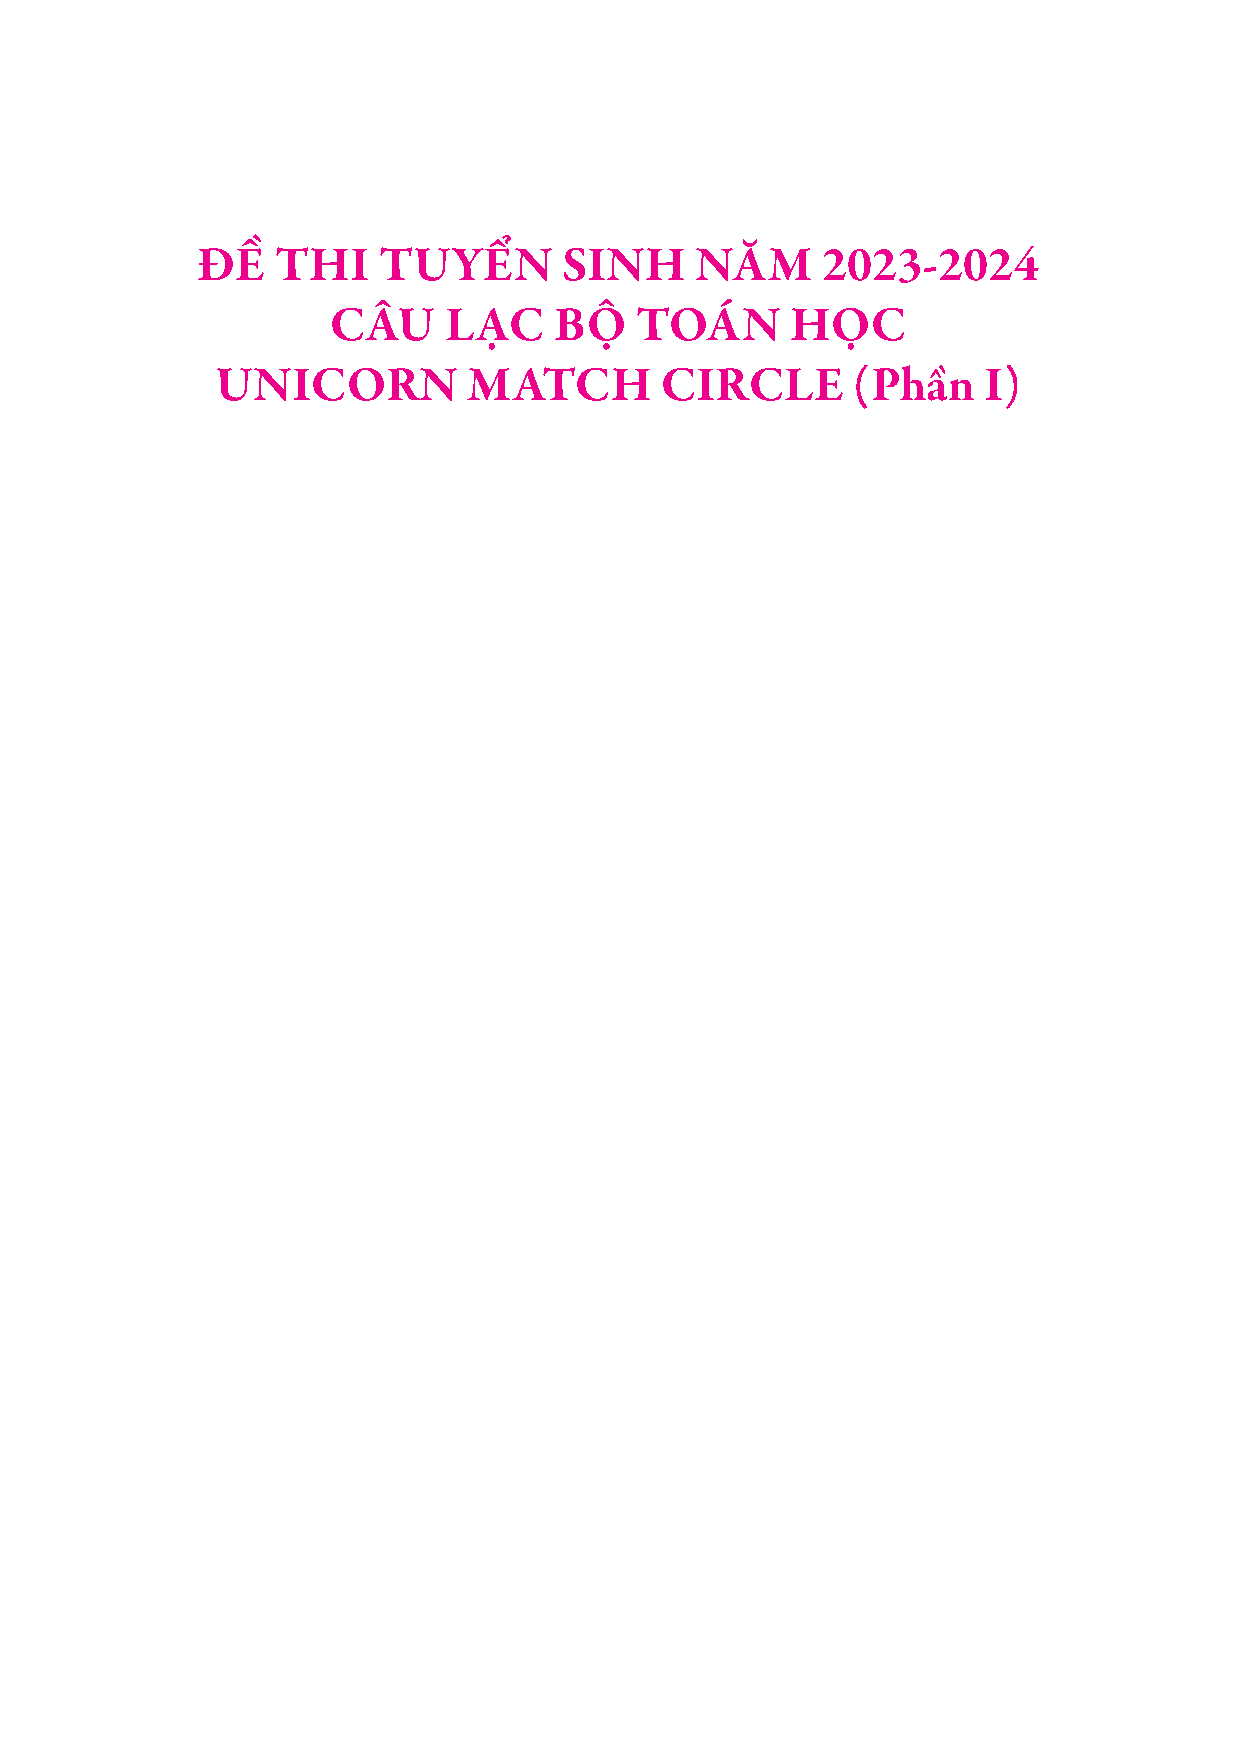
\includegraphics[scale=1]{../tieude1.pdf}}} 
\centering
\endgroup
\vspace*{160pt}

\begin{multicols}{2}
	\textbf{\color{toancuabi}Bài} $\pmb{1.}$ Cho đa giác lồi $n$ cạnh có $65$ đường chéo. Tìm giá trị của $n$.
	\vskip 0.1cm
	\textbf{\color{toancuabi}Bài} $\pmb{2.}$ Tìm số nguyên dương $n$ sao cho $7n$ chia hết cho $n+1$.
	\vskip 0.1cm
	\textbf{\color{toancuabi}Bài} $\pmb{3.}$ Một tờ giấy hình tròn được vẽ các đường tròn màu xanh, đỏ và vàng cùng tâm. Nếu cắt dọc theo các đường màu xanh, bạn nhận được $10$ mảnh, nếu cắt dọc theo các đường màu đỏ bạn nhận được $12$ mảnh và nếu cắt theo các đường màu vàng bạn nhận được $18$ mảnh. Hỏi nếu cắt theo tất cả các đường cả xanh, đỏ, vàng thì bạn nhận được bao nhiêu mảnh giấy?
	\vskip 0.1cm
	\begin{figure}[H]
		\vspace*{-5pt}
		\centering
		\captionsetup{labelformat= empty, justification=centering}
		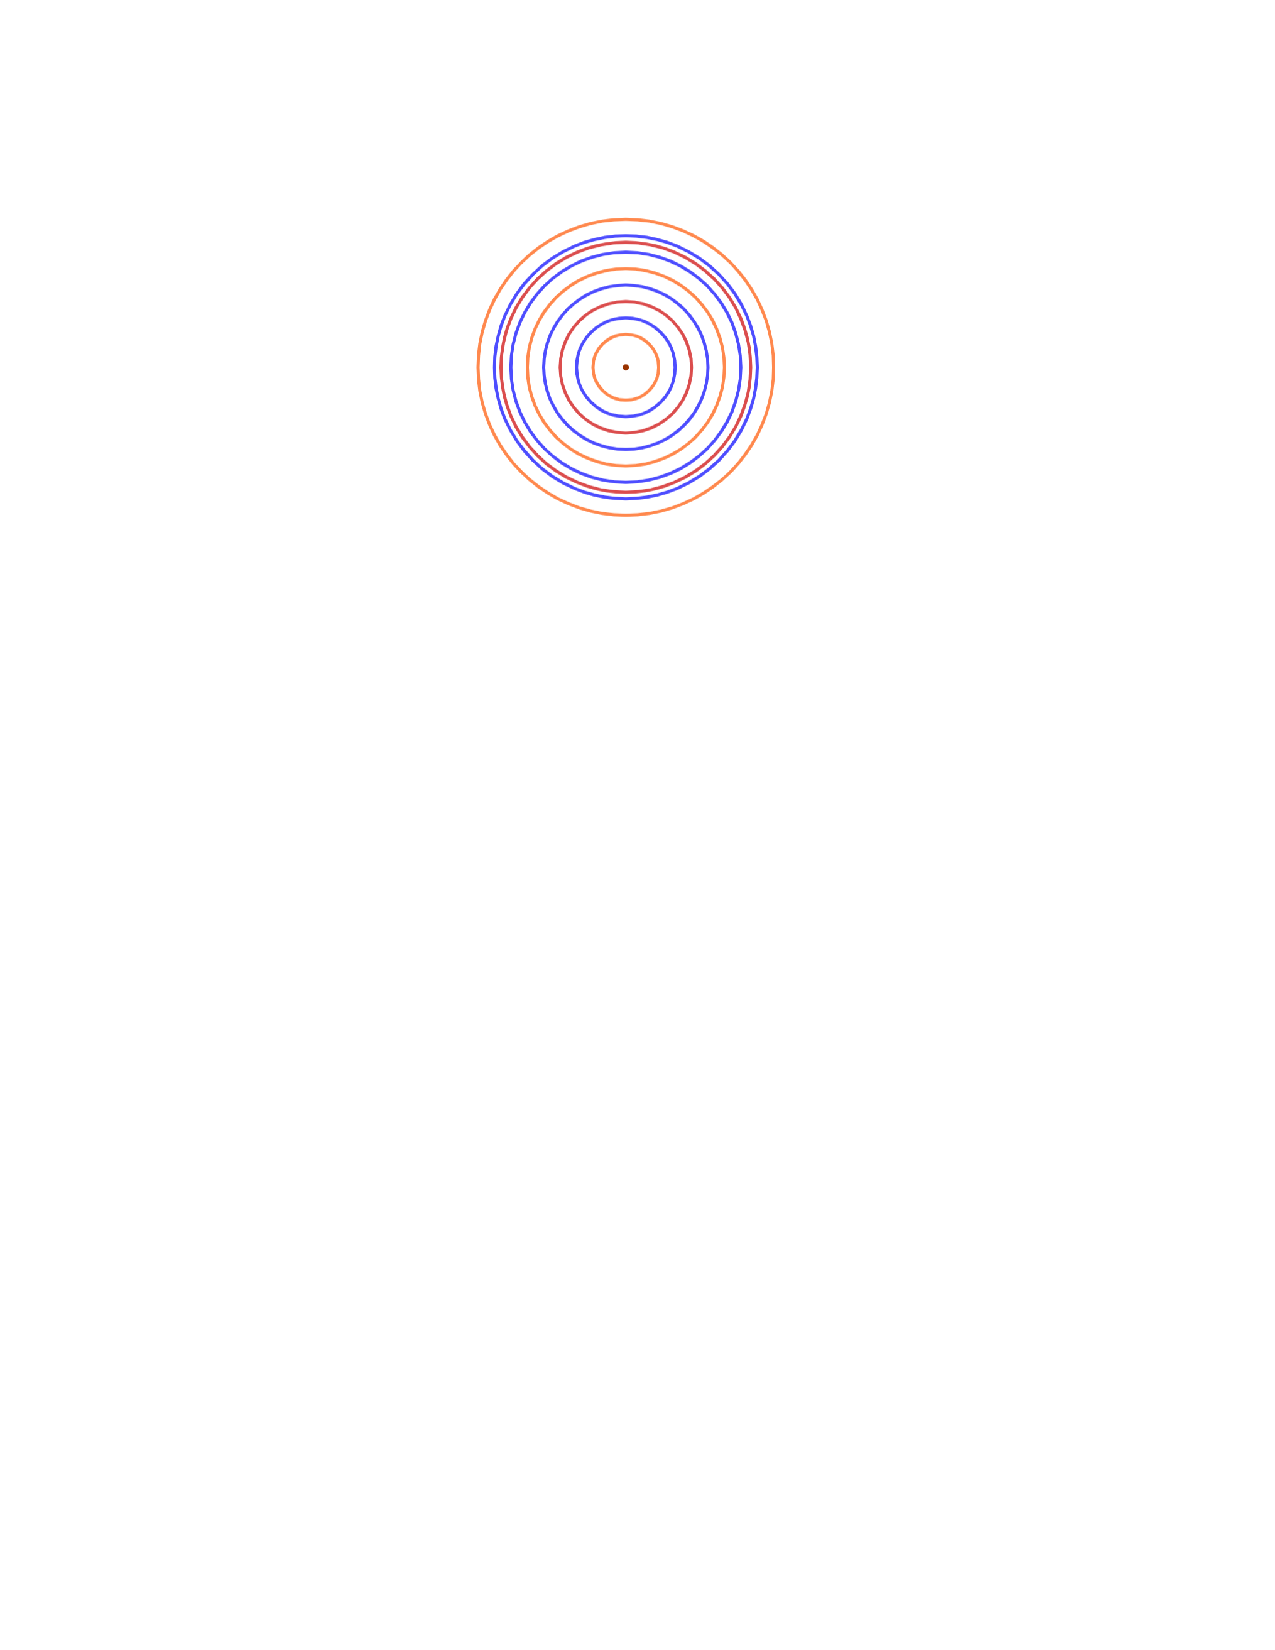
\includegraphics[width= 0.6\linewidth]{bai3}
		\caption{\small\textit{\color{toancuabi}Hình vẽ mang tính chất minh họa.}}
		\vspace*{-10pt}
	\end{figure}
	\textbf{\color{toancuabi}Bài} $\pmb{4.}$ Tìm số có $2$ chữ số $AB$ thỏa mãn điều kiện như
	phép tính bên.
	\begin{table}[H]
		\vspace*{-5pt}
		\centering
		\captionsetup{labelformat= empty, justification=centering}
		\begin{tabular}{ccc}
			&$A$&$B$\\
			$\times$& &$A$\\
			\hline
			$B$&$A$&$A$\\
		\end{tabular}	
%		\caption{\small\textit{\color{}.}}
		\vspace*{-10pt}
	\end{table}
	\textbf{\color{toancuabi}Bài} $\pmb{5.}$ Trong vườn của bác nông dân có $2024$ cây đào. Có đúng một nửa số cây đào đang ra hoa và $\frac{1}{4}$ số cây đào đang ra quả (trong số đó có một số cây đang ra cả hoa và quả). Biết rằng có $1000$ cây đào chưa ra cả hoa lẫn quả. Hỏi có bao nhiêu cây đào đã ra cả hoa và quả?
	\vskip 0.1cm
	\textbf{\color{toancuabi}Bài} $\pmb{6.}$ Tình chữ số tận cùng của $A = 2^{2021} + 3^{2022} + 4^{2023} + 7^{2024.}$
	\vskip 0.1cm
	\textbf{\color{toancuabi}Bài} $\pmb{7.}$ Câu lạc bộ tem có $40$ thành viên. Có $25$ người có không ít hơn $25$ cái tem và có $26$ người có ít hơn $26$ cái tem. Hỏi có bao nhiêu người có đúng $25$ cái tem?
	\vskip 0.1cm
	\textbf{\color{toancuabi}Bài} $\pmb{8.}$ Trên bảng ghi $21$ số chẵn liên tiếp. Bạn Phong xóa đi $1$ số và thấy tổng của các số còn lại bằng $2024$. Hỏi Phong đã đi xóa đi số nào?
	\vskip 0.1cm
	\textbf{\color{toancuabi}Bài} $\pmb{9.}$ Cho hình lập phương $ABCDEFGH$ như hình vẽ. Hỏi có bao nhiêu tam giác vuông có $3$ đỉnh là các đỉnh của hình lập phương đã cho.
	\begin{figure}[H]
		\vspace*{-5pt}
		\centering
		\captionsetup{labelformat= empty, justification=centering}
		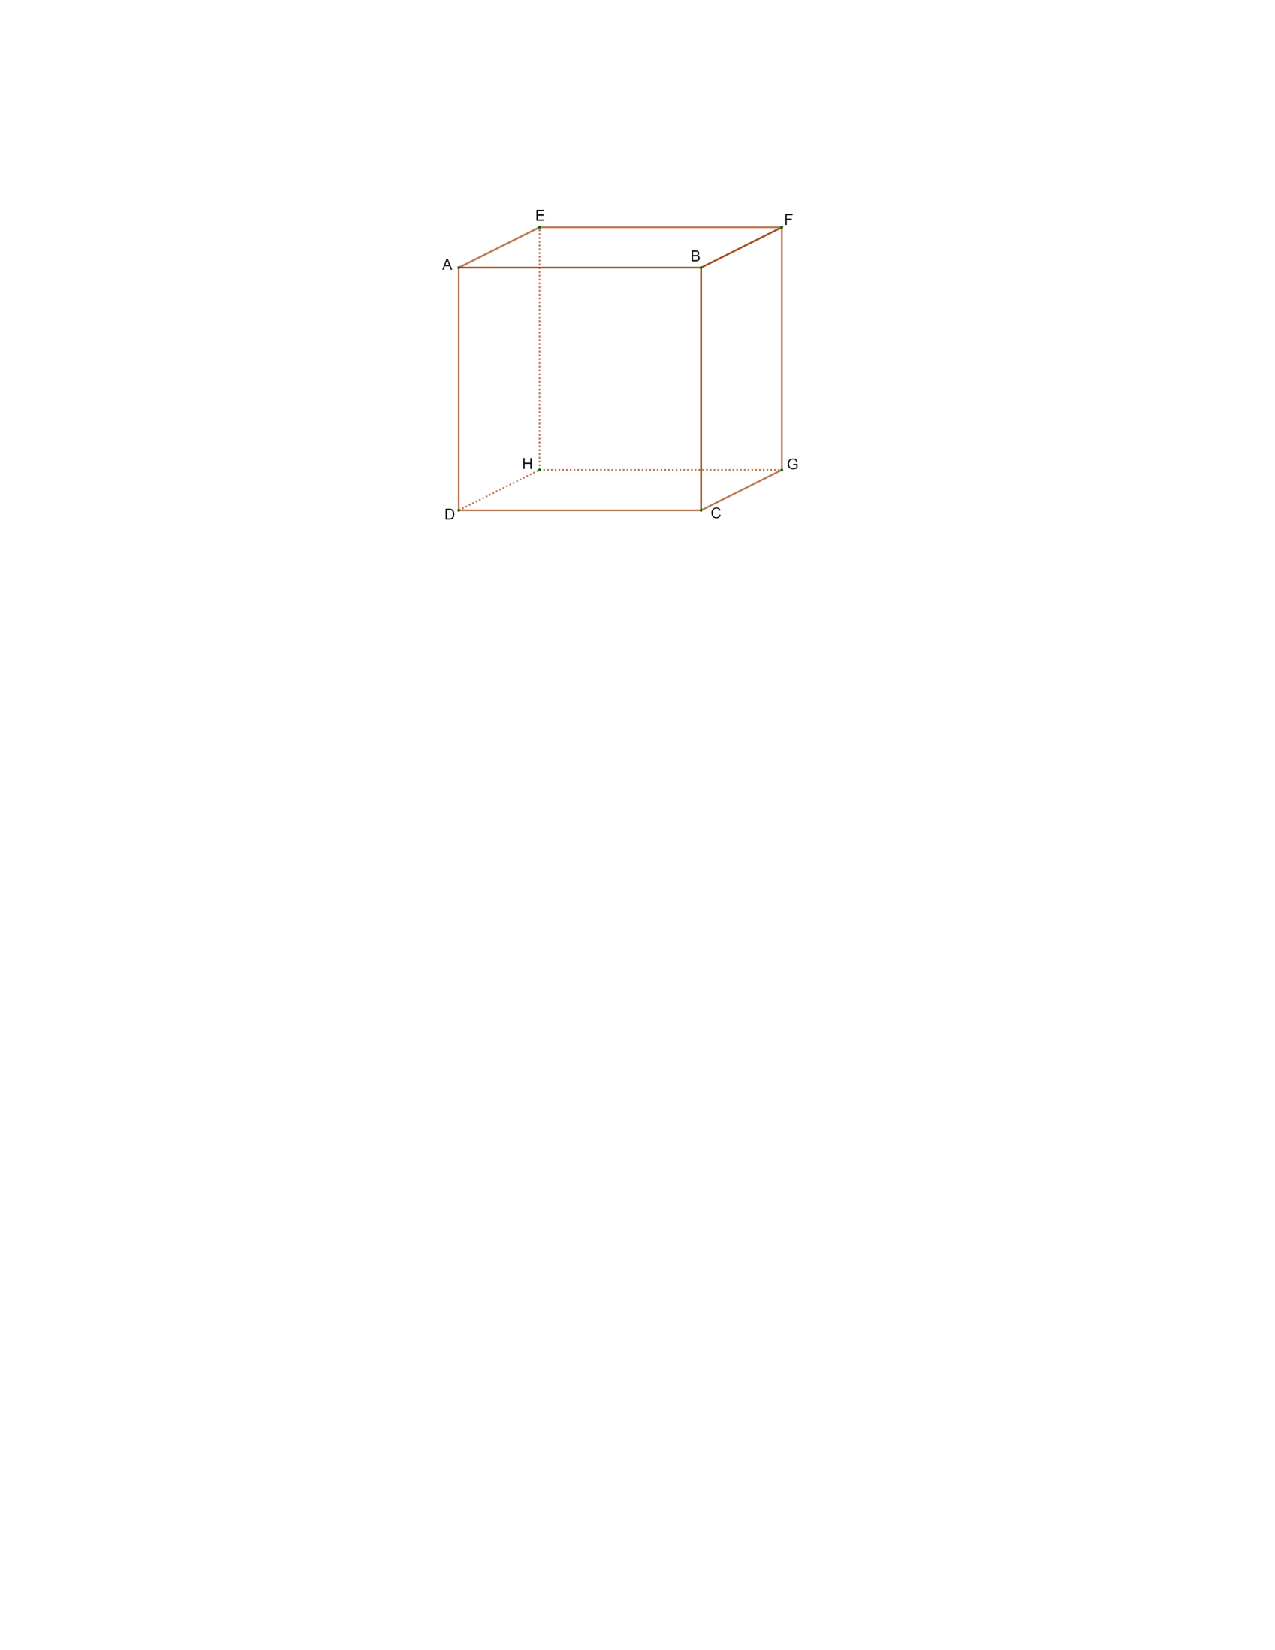
\includegraphics[width= 0.7\linewidth]{bai9}
%		\caption{\small\textit{\color{}}}
		\vspace*{-10pt}
	\end{figure}
	\textbf{\color{toancuabi}Bài} $\pmb{10.}$ Cho hình vuông $ABCD$ và đường gấp khúc $CMNPQB$ như hình vẽ. Biết các độ dài $DM$, $MN$,
	$NP$, $PQ$ và $QB$ là $2$, $2$, $2$, $1$, $3$ đơn vị. Tính diện tích
	hình vuông $ABCD$.
	\begin{figure}[H]
		\vspace*{-5pt}
		\centering
		\captionsetup{labelformat= empty, justification=centering}
		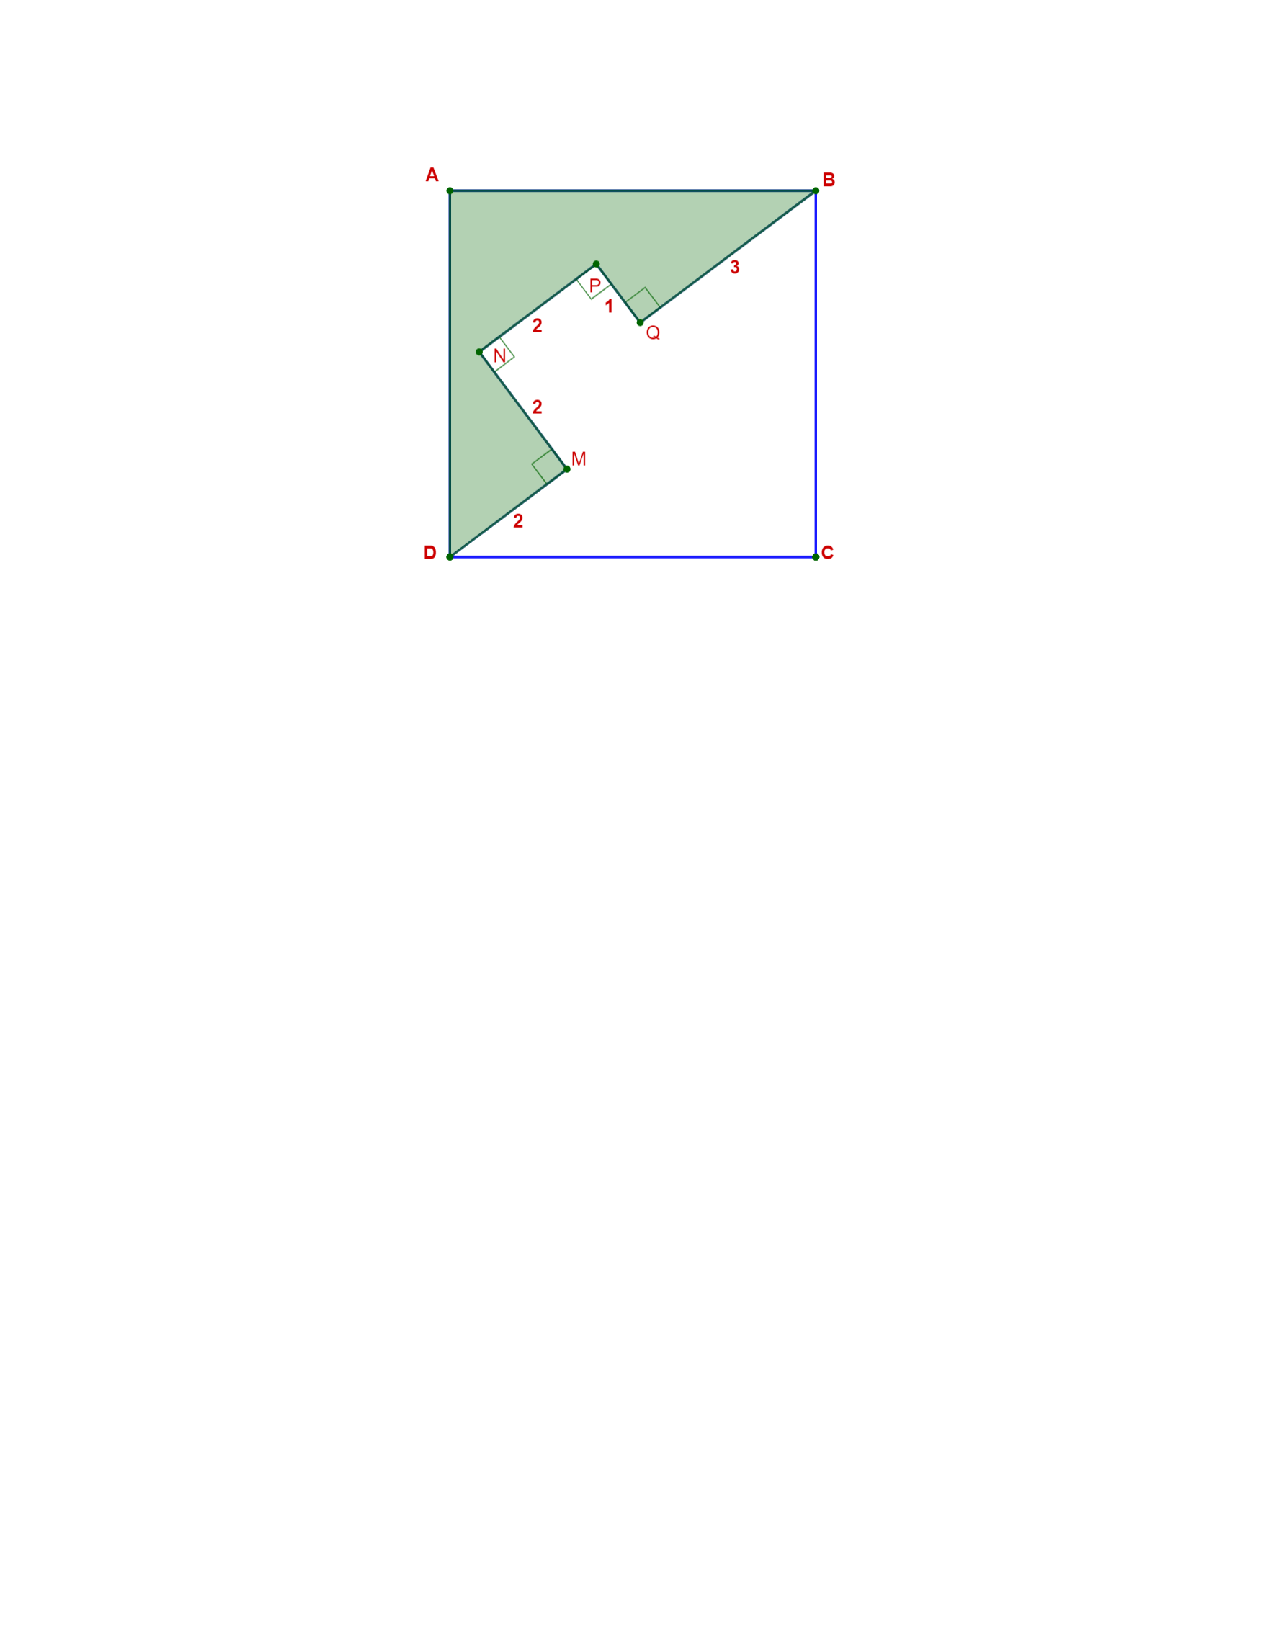
\includegraphics[width= 0.7\linewidth]{bai10}
		%		\caption{\small\textit{\color{}}} 
		\vspace*{-10pt}
	\end{figure}
	\textbf{\color{toancuabi}Bài} $\pmb{11.}$ Có $15$ bạn nhỏ vào rừng hái nấm, không có $2$ bạn nào hái được cùng số nấm. Hỏi các bạn cần hái nhiều nhất bao nhiêu cái nấm để chắc chắn rằng có $2$ bạn hái được số nấm như nhau?
	\vskip 0.1cm
	\textbf{\color{toancuabi}Bài} $\pmb{12.}$ Một cái khóa số có mã gồm $3$ chữ số với các thông tin như hình bên. Bạn hãy phá khóa và cho biết mã của khóa là số nào?
	\begin{figure}[H]
		\vspace*{-5pt}
		\centering
		\captionsetup{labelformat= empty, justification=centering}
		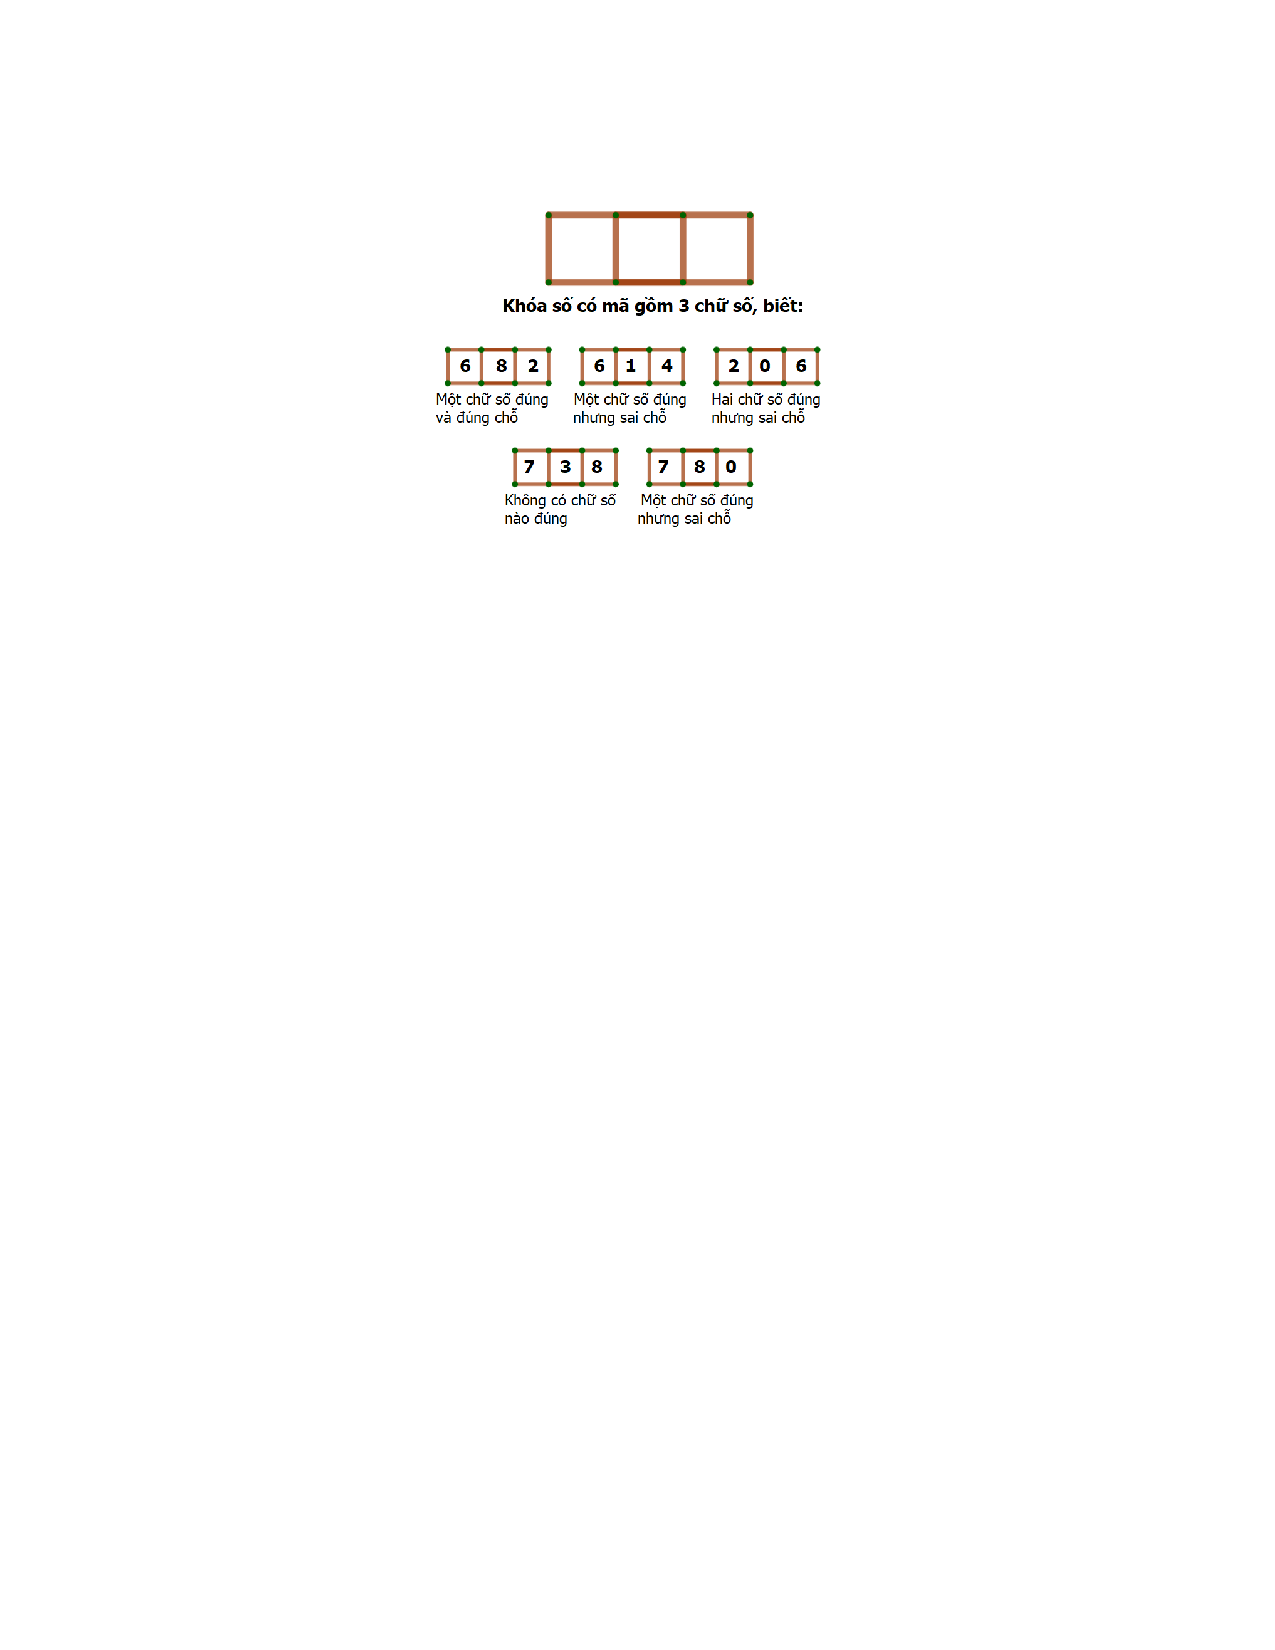
\includegraphics[width= 1\linewidth]{bai12}
%		\caption{\small\textit{\color{}}}
		\vspace*{-15pt}
	\end{figure}
	\textbf{\color{toancuabi}Bài} $\pmb{13.}$ Tính giá trị của $S$.
	\begin{align*}
		S =& \frac{1}{1\times 2 \times 5} + \frac{1}{2\times 5 \times 6} + \frac{1}{6\times9\times 10} \\
		&+ \cdots + \frac{1}{26 \times 29 \times 30} + \frac{1}{29\times 30 \times 33}
	\end{align*}
	\textbf{\color{toancuabi}Bài} $\pmb{14.}$ Có bao nhiêu tam giác vuông có đỉnh là các điểm trong lưới ô vuông $4\times 4$ (chấm) như hình vẽ.
	\begin{figure}[H]
		\vspace*{-5pt}
		\centering
		\captionsetup{labelformat= empty, justification=centering}
		\begin{tikzpicture}[toancuabi,scale=0.9]
			\draw[fill=toancuabi] (0,0) circle (1.5pt);
			\draw[fill=toancuabi] (0,1) circle (1.5pt);
			\draw[fill=toancuabi] (0,2) circle (1.5pt);
			\draw[fill=toancuabi] (0,3) circle (1.5pt);
			\draw[fill=toancuabi] (0,3) circle (1.5pt);
			\draw[fill=toancuabi] (1,0) circle (1.5pt);
			\draw[fill=toancuabi] (1,1) circle (1.5pt);
			\draw[fill=toancuabi] (1,2) circle (1.5pt);
			\draw[fill=toancuabi] (1,3) circle (1.5pt);
			\draw[fill=toancuabi] (2,0) circle (1.5pt);
			\draw[fill=toancuabi] (2,1) circle (1.5pt);
			\draw[fill=toancuabi] (2,2) circle (1.5pt);
			\draw[fill=toancuabi] (2,3) circle (1.5pt);
			\draw[fill=toancuabi] (3,0) circle (1.5pt);
			\draw[fill=toancuabi] (3,1) circle (1.5pt);
			\draw[fill=toancuabi] (3,2) circle (1.5pt);
			\draw[fill=toancuabi] (3,3) circle (1.5pt);
		\end{tikzpicture}
		\vspace*{-5pt}
	\end{figure}
	\textbf{\color{toancuabi}Bài} $\pmb{15.}$ Trong hình vẽ đã cho, ở hàng cuối cùng được viết các số nguyên dương khác nhau. Mỗi ô ở trên có giá trị bằng tích của $2$ ô nằm ngay dưới nó.
	Tính giá trị nhỏ nhất của $X$.
	\begin{figure}[H]
		\vspace*{-5pt}
		\centering
		\captionsetup{labelformat= empty, justification=centering}
		\begin{tikzpicture}[toancuabi,scale=0.85]
			\draw (0,0) grid (5,1);
			\draw (0.5,1) rectangle (4.5,2);
			\draw (1,2) grid (4,3);
			\draw (1.5,3) rectangle (3.5,4);
			\draw (2.5,3) -- (2.5,4) (1.5,1) -- (1.5,2) (2.5,1) -- (2.5,2) (3.5,1) -- (3.5,2);
			\draw (2,4) grid(3,5);
		\end{tikzpicture}
		\vspace*{-10pt}
	\end{figure}
	\textbf{\color{toancuabi}Bài} $\pmb{16.}$ Ba số được chọn ngẫu nhiên từ $20$ số $\{1,2,3,..,20\}$. Xác suất để tổng ba số này chia hết cho $3$ là bao nhiêu?
	\vskip 0.1cm
	\textbf{\color{toancuabi}Bài} $\pmb{17.}$ Có bao nhiêu số nguyên dương không lớn hơn $2024$ và nguyên tố cùng nhau với $2024$.
	\vskip 0.1cm
	\textit{(Hai số tự nhiên $(a,b)$ nguyên tố cùng nhau nếu $a$ và $b$ có ước chung duy nhất là $1$)}.
	\vskip 0.1cm
	\textbf{\color{toancuabi}Bài} $\pmb{18.}$ Cho tam giác $ABC$ có diện tích bằng $630$
	cm$^2$ như hình vẽ. Biết rằng $BD=DE=EC$,
	$CF=FG=GA$. Tính diện tích phần tô đậm.
	\begin{figure}[H]
		\vspace*{-5pt}
		\centering
		\captionsetup{labelformat= empty, justification=centering}
		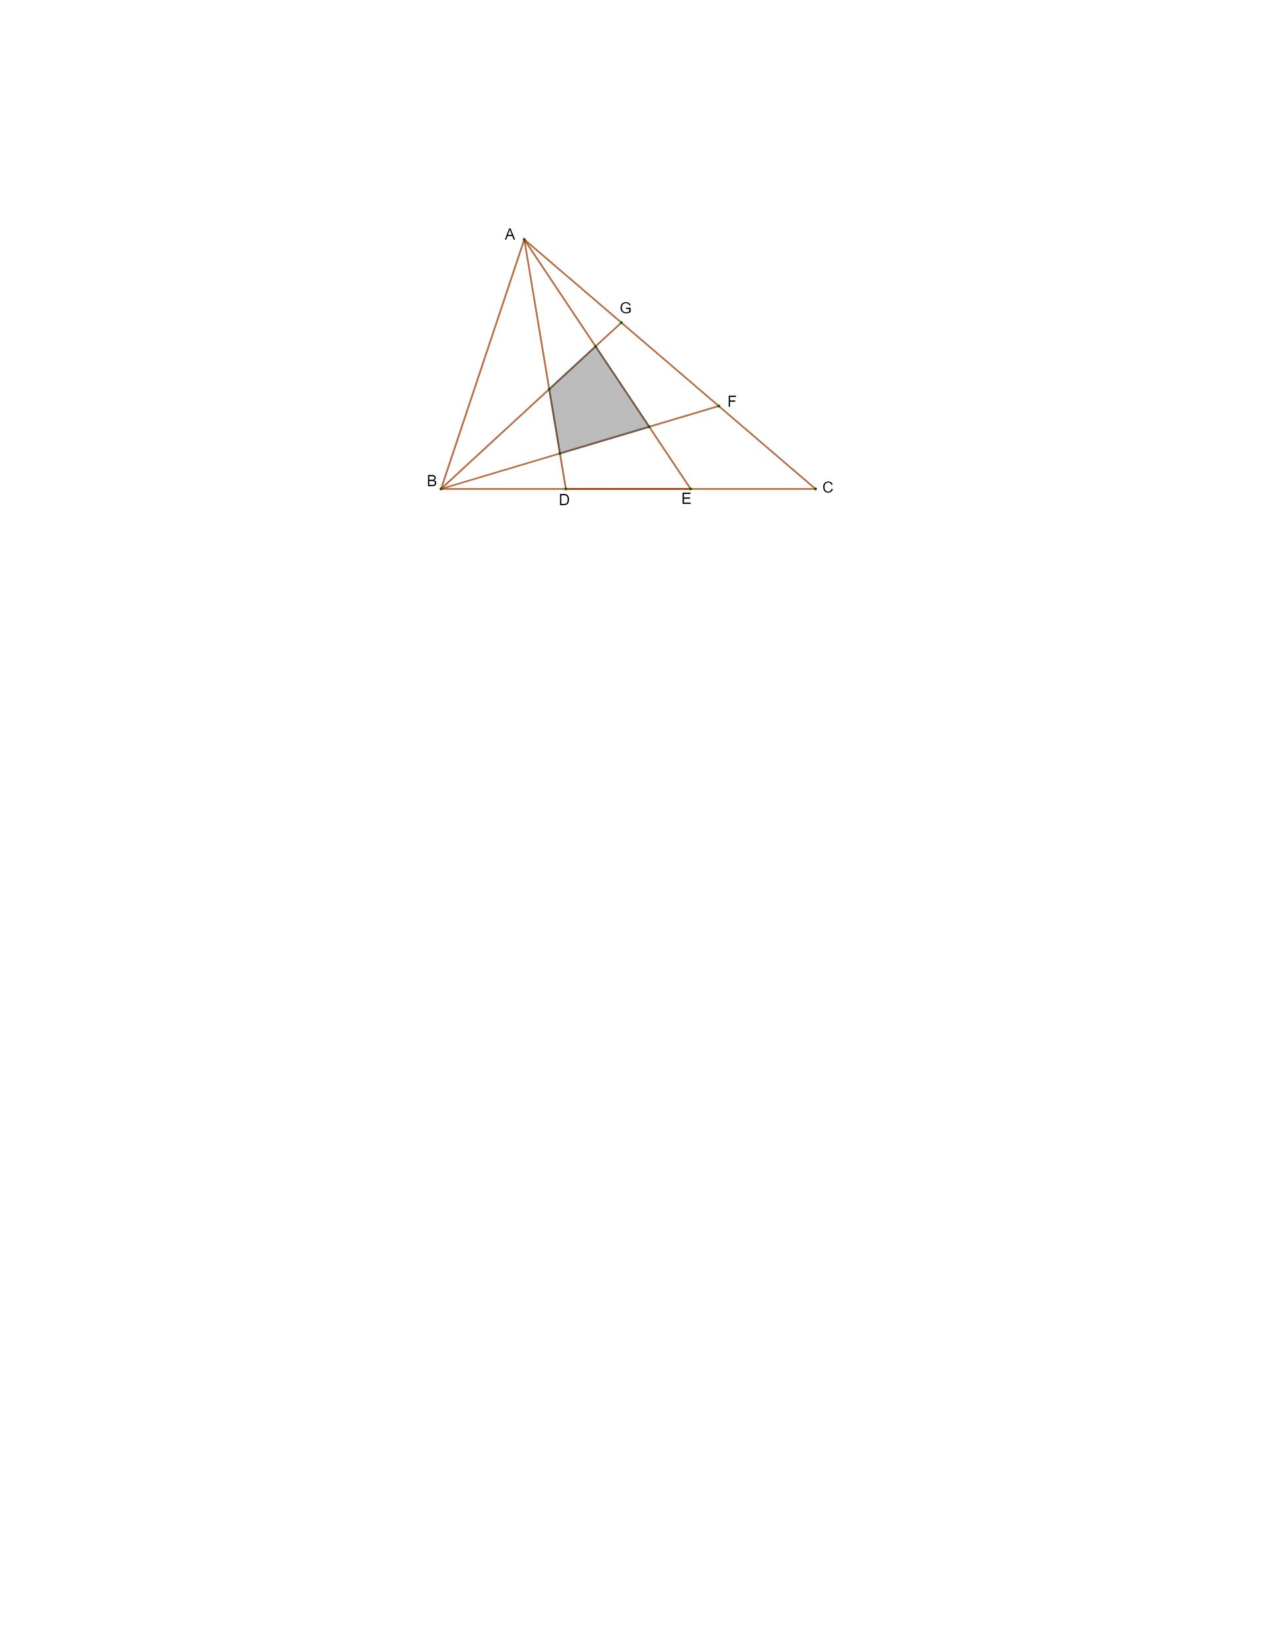
\includegraphics[width= 1\linewidth]{bai18}
%		\caption{\small\textit{\color{}}}
		\vspace*{-10pt}
	\end{figure}
	\textbf{\color{toancuabi}Bài} $\pmb{19.}$ Có bao nhiêu số có $4$ chữ số chia hết cho $9$ mà không chứa chữ số $9$?
	\vskip 0.1cm
	\textbf{\color{toancuabi}Bài} $\pmb{20.}$ Мột con ếch nhảy qua các đỉnh của tam giác $ABC$, mỗi lần nhảy qua một trong các đỉnh lân cận. Hỏi có bao nhiêu cách con ếch có thể đi từ $A$ và quay về $A$ sau $6$ lần nhảy?
\end{multicols}